\documentclass{ML}
\usepackage{amsthm}
\usepackage{fontspec}
\usepackage[ruled,linesnumbered]{algorithm2e}

\setmonofont{Iosevka Nerd Font Mono}

\newtheorem{theorem}{定理}
% \newtheorem{proof}{证明}

% 姓名,学号
\infoauthor{冯云龙}{1160300202}

% 课程类型,实验名称
\infoexp{选修}{多项式拟合正弦曲线}

\begin{document}
\maketitle

\tableofcontents
\newpage

\section{实验目的}

\begin{enumerate}
	\item 掌握最小二乘法求解(无惩罚项的损失函数)
	\item 掌握加惩罚项 (2范数) 的损失函数优化
	\item 掌握梯度下降法
	\item 掌握共轭梯度法
	\item 理解过拟合
	\item 掌握克服过拟合的方法(加惩罚项、增加样本)
\end{enumerate}

\section{实验要求及实验环境}

\subsection{实验要求}

\begin{enumerate}
	\item 生成数据、加入噪声
	\item 用高阶多项式拟合曲线
	\item 用解析解求解两种loss的最优解(无正则项和有正则项)
	\item 优化方法求解最优解(梯度下降、共轭梯度)
	\item 用不同数据集,不同超参数,不同的多项式阶数,比较实验效果
\end{enumerate}

\subsection{实验环境}

\begin{itemize}
	\item 操作系统:Manjaro Linux x64
	\item 编程语言:Julia
	\item 绘图工具包:Plots.jl
	\item IDE:Atom (Juno)
\end{itemize}

\section{设计思想}

线性模型(linear model)试图学得一个通过属性的线性组合来进行预测的函数。其形式简单、易于建模,许多功能更为强大的非线性模型可在线性模型的基础上通过引入层级结构或高维映射而得。

我们的目的就是在拟合数据集的函数基础上对新样本进行预测,当然我们会希望对原数据和新数据都能够很好的进行预测,那么我们就需要一种方法来评测预测值和实际值的差异程度。

\subsection{算法原理}

\begin{table}[H]
	\centering
	\begin{tabular}{ccc}
		\\ \hline
		符号                          & 释义           & 注释        \\ \hline
		\(X = x^{1},x^{2},…,x^{m}\)   & 样本集         &             \\
		\(x^i = x_1^i,x_2^i,…,x_n^i\) & 样本属性集     & 通常会包含b \\
		\(Y = y^{1},y^{2},…,y^{m}\)   & 标签集         &             \\
		\(W = w^{1},w^{2},…,w^{n}\)   & 依赖关系描述集 &
		\\ \hline
	\end{tabular}
\end{table}

我们当然希望我们得到的线性模型\(\hat{Y} = X \hat{W}\),通过计算得到的\(\hat{Y}\)与实际的\(Y\)比较相近,那么我们可以设置一个量来表示\(\hat{Y}\)和\(Y\)的相近程度。

即:

\[\arg \min_W \sum^m_{i=1}(y^i - x^i\hat{w})^2\]

我们已知数据集

\[D = {(x^1,y^1),(x^2,y^2),…,(x^m,y^m)}\]

那么我们就可以设置误差函数\(E_{\hat{W}}\),来描述我们的预测值与实际值的偏差情况,则有:
\[E_{\hat{W}} = \frac{1}{length(X)} ∑(y - x \hat{w})^2\]

把他们换成矩阵的形式:

\[x^i = \begin{bmatrix}
		x^i_1 & x^i_2 & x^i_3 & x^i_4 & … & x^i_n
	\end{bmatrix}\]

\[X = \begin{bmatrix}
		x^1 \\ x^2 \\ x^3 \\ x^4 \\ \vdots \\  x^m
	\end{bmatrix}
	Y = \begin{bmatrix}
		y^1 \\ y^2 \\ y^3 \\ y^4 \\ \vdots \\  y^m
	\end{bmatrix}
	W = \begin{bmatrix}
		w^1 \\ w^2 \\ w^3 \\ w^4 \\ \vdots \\  w^n
	\end{bmatrix}\]

那么我们就有了

\[E_{\hat{W}} = \frac{1}{length(X)} (Y - X \hat{W})^T(Y - X \hat{W})\]

我们的目标是找到一个合适的\(W\)使得误差函数值最小,那么我们用误差函数对\(W\)求导:

\[\frac{∂E_{\hat{W}}}{∂\hat{W}} = \frac{1}{length(X)} 2X^T(X\hat{W} - Y)\]

既然是要求最小值,那么我们令导数为零,则有:

\[\frac{∂E_{\hat{W}}}{∂\hat{W}} = 0 → \hat{W} = (X^TX)^{-1}X^TY\]

\subsubsection{梯度下降}

我们希望导数为零,那么自然要向导数的反方向移动,而后我们则有:

\[\hat{W} = \hat{W} - \alpha\frac{∂E_{\hat{W}}}{∂\hat{W}}\]

随机梯度下降是梯度下降的一种特例,即使用数据集中的某一部分数据进行训练,可以大大减少内存的需求。

\subsubsection{共轭梯度下降}

首先我们规定以下符号

\begin{table}[H]
	\centering
	\begin{tabular}{ccc}
		\hline
		符号       & 释义     & 注释                             \\ \hline
		\(A\)      & 系数矩阵 &                                  \\
		\(x\)      & 变量矩阵 &                                  \\
		\(r\)      & 残差     & 上次优化过后,距离最优点的残余量 \\
		\(\alpha\) & 优化距离 & 即在优化方向上步进的距离         \\
		\(p\)      & 优化方向 & 即下一次优化的方向               \\ \hline
	\end{tabular}
\end{table}

\begin{theorem}
	\(A\)为\(n×n\)对称正定矩阵,\(p_1,p_2,…,p_m\)为\(A\)共轭的非零向量,则这一组向量线性独立。
\end{theorem}

\begin{proof}
	设有一组实数\(a_1,a_2,…,a_m\)使得\(a_1p_1+a_2p_2+…+a_mp_n = 0\)。用\(p_i^TA\)左乘上式,得到\(m\)个等式。又\(p_i^T A p_j = 0,(i≠q)\),得到\(a_ip_i^TAp_i = 0,(i = 1,2,…,m)\)。由于正定矩阵的二次型大于0,故有\(p_i^TAp_i > 0\),则\(a_i=0,(i = 1,2,…,m)\),由线性五官向量组的定义,找不到一组非零实数\(a_1,a_2,…,a_m\)使得\(a_1p_1+a_2p_2+…+a_mp_n = 0\),则\(p_1,p_2,…,p_m\)为线性无关方向组。
\end{proof}

\begin{theorem}
	\(A\)为\(n×n\)对称正定矩阵,\(p_1,p_2,…,p_n\)为\(A\)共轭的非零向量,则从任意一点\(x_0\)出发,相继以\(p_1,p_2,…,p_n\)为搜索反响进行一次一维搜索,则经过\(n\)次搜索后收敛于正定二次函数极小值问退的极小值点\(x^*\)。
\end{theorem}

\begin{proof}
	在以\(A-\)共轭方向组为更新方向时,梯度\(\nabla f_k\)与更新方向\(d_0,d_1,\dots,d_{k-1}\)都正交。从\(x_0\)出发,依次沿 着\(p_0,p_1,…,p_{k-1}\)为搜索反响进行一次一维搜索,点的更新步长为最优步长\(\alpha_0,\alpha_2,\dots,\alpha_{k-1}\)。

	\[\begin{array}{lll}
			x_k & = x_{k-1} + \alpha_{k-1}p_{k-1}                           \\
			    & = x_i + \sum_{j=i}^{k-1}\alpha_{j}p_{j} & (i = 0,1,…,k-1)
		\end{array}\]

	在以\(A-\)共轭方向组为更新方向时,\(p_n\)与更新方向\(p_0,…,p_{k-1}\)均共轭正交。从\(x_0\)出发,依次沿着\(p_0,…,p_{k-1}\)进行一维搜索,点的更新步长为最优步长\(\alpha_0,…,\alpha_{k-1}\)。

	\[\begin{array}{lll}
			x_k & = x_{k-1} + \alpha_{k-1}p_{k-1}                           \\
			    & = x_i + \sum_{j=i}^{k-1}\alpha_{j}p_{j} & (i = 0,1,…,k-1)
		\end{array}\]

	\[\begin{array}{ll}
			g_k      & = ∇f(x_k)                                            \\
			         & = Ax_k - b                                           \\
			         & = Ax_{i} + \sum^{k-1}_{j=i}\alpha_jAp_j - b          \\
			         & = g_{i+1} + \sum^{k-1}_{j=i}\alpha_jAp_j             \\
			p_i^Tg_k & = p_i^Tg_{i+1} + \sum_{j=i+1}^{k-1}\alpha_jp_i^TAp_j
		\end{array}\]

	我们每次都优化到当前行进方向的最优点,则有\(\frac{df(x_i + \alpha p_i)}{d\alpha}|_{\alpha=\alpha_i} = 0\),而后我们可以得到\(p_i^Tg(x_{i+1}) = 0\)。由\(p_0,p_1,…,p_{k-1}\) 为\(A-\)共轭组我们得到\(\sum_{j=j+1}^{k-1}\alpha_jp_i^TAp_j = 0\)。所以我们有\(p_ig_k = 0,(i=0,1,…,k-1)\)。

	即对于\(A-\)共轭组来说,\(p_i(i=0,1,…,k-1)\)和\(g_k\)是正交的。当\(k=n\)的时候,\(g_n\)与\(p_i(i=0,1,…,n-1)\)正交,而\(p_i(i=0,1,…,n-1)\)之间是线性无关的。那么\(g_n\)与\(n\)个线性向量无关,则有\(g_n=0\),所以\(x_n\)是该无约束凸二次规划问题的最优解。

	看一下我们上边的公式,我们需要得到每一步需要更新的步长和方向。我们引入残差\(r_k = b - Ax_k\),它描述了我们在第k步优化的方向。由于之前提到我们每次更新的方向之间都是共轭的,在该方向上,我们同样直接一次优化到位,那么下一次优化的方向与之前优化的方向都是共轭的,那么即是说,我们这次优化的方向需要从当前残差与之前优化过的方向中构建,我们使用当前残差减去之前优化方向的分量:

	\[\begin{array}{ll}
			p_k & = r_k - \sum_{i < k}\frac{p_i^TAr_k}{p_i^TAp_i}p_{i}
		\end{array}\]

	在这个方向上取\(\frac{df(x_k + \alpha p_k)}{d\alpha}|_{\alpha=\alpha_k} = 0\),可以得出:

	\[\alpha_k = \frac{p_k^T r_k}{p_k^T A p_k}\]

\end{proof}

在数据量很小的时候,我们的估计函数能力过于强大,使得在训练集上的误差极小,但是得到的模型也是异常复杂,使得我们模型的泛化能力极低,在测试集上的误差又极大,通俗来说,就是只学会了学过的东西,但是对新的东西不能很好的处理。

那么我们希望可以限制模型的复杂度,当然,首先我们需要知道什么量和模型的复杂度相关,在实验过程中,我们会发现$W$的值越大,模型越复杂,那么我们就可以对此加以限制,使得$W$不能取这么大的值,于是我们就有:

$$E_{\hat{W}} = \frac{1}{length(X)} (∑(y - x \hat{w})^2 + λ∑\hat{w}^2)$$

其中λ为正则项在进行拟合过程中占得比重,类似的,我们可以得到:

$$E_{\hat{W}} = \frac{1}{length(X)} ((Y - X \hat{W})^T(Y - X \hat{W}) + λ\hat{W}^T\hat{W})$$

$$\frac{∂E_{\hat{W}}}{∂\hat{W}} = \frac{2}{length(X)} (X^T(X\hat{W} - Y) + λ\hat{W})$$

$$\frac{∂E_{\hat{W}}}{∂\hat{W}} = 0 → \hat{W} = (X^TX + λI)^{-1}X^TY$$

\subsection{一些优化方案}

\subsubsection{动量(Momentum)}

动量来源于牛顿定律,基本思想是为了找到最优加入“惯性”的影响,当误差曲面中存在平坦区域,SGD就可以更快的学习。

$$V = β * V - α\frac{∂E_{\hat{W}}}{∂\hat{W}}$$
$$\hat{W} = \hat{W} + V$$

\subsubsection{权值衰减(Weight Decay)}

在实际应用中,为了避免网络的过拟合,必须对价值函数(Cost function)加入一些正则项,在SGD中加入$\alpha \lambda \omega _{i}$ 这一正则项对这个Cost function进行规范化:

权值衰减的使用既不是为了提高收敛精确度也不是为了提高收敛速度,其最终目的是防止过拟合。在损失函数中,weight decay是放在正则项(regularization)前面的一个系数,正则项一般指示模型的复杂度,所以weight decay的作用是调节模型复杂度对损失函数的影响,若weight decay很大,则复杂的模型损失函数的值也就大。

$$\omega_{i+1}\leftarrow  \omega_{i} - \alpha \frac{\partial E}{\partial \omega_{i}} - \alpha \lambda \omega _{i}$$

上面这个公式基本思想就是减小不重要的参数对最后结果的影响,网络中有用的权重则不会收到Weight decay影响。

\subsubsection{退火(leanrning Rate Decay)}

在极值点附近,求解会由于学习率过大,导致解在极值点两侧摇摆,收敛速度变慢,很自然的想法是在极值点附近自动降低学习率。

在使用梯度下降法求解目标函数$E_{W}$的极小值时,更新公式为$W=W+ v$,其中每次$W$的更新量$v$为$v = - \frac{∂E_{W}}{∂W} * lr$,$\frac{∂E_{W}}{∂W}$为目标函数$E_{W}$对$W$的一阶导数。可以想到,如果能够让学习率随着迭代周期不断衰减变小,那么搜索时迈的步长就能不断减少以减缓震荡。学习率衰减因子由此诞生:


$$lr_i = lr_{start} * \frac{1}{1 + δ * i}$$

上面的公式即为学习率衰减公式,其中$lr_i$为第i次迭代时的学习率,$lr_{start}$为原始学习率,$δ$为一个介于[0.0, 1.0]的小数。
从公式上可看出:

\begin{enumerate}
	\item $δ$越小,学习率衰减地越慢,当$δ = 0$时,学习率保持不变。
	\item $δ$越大,学习率衰减地越快,当$δ = 1$时,学习率衰减最快。
\end{enumerate}

\subsection{算法的实现}

\subsubsection{梯度下降}

\begin{algorithm}[H]
	\caption{随机梯度下降}\label{algorithm}

	\KwData{自变量\(X\), 标签\(Y\), 正则化系数\(\lambda\),需要的精度\(Error\)}
	\KwResult{相关系数矩阵 \(\hat{W}\)}

	Init \(\hat{W},V\)

	\(err \leftarrow \frac{\sum_{\Delta y \in X^T\hat{W} - Y}\Delta y^2}{length(Y)}\)

	\While{\(err > Error\)}{
		\(\partial E_W \leftarrow \frac{2}{length(Y)} (X^T X \hat{W} - Y + \lambda \hat{W})   \) \;
		\(lr_i \leftarrow \frac{\alpha}{1 + lr_{decay} * i}\) \;
		\(v \leftarrow Momentum * v - lr_i * \partial E_W \) \;
		\(\hat{W} \leftarrow \hat{W} + v\) \;
		\(err \leftarrow \frac{\sum_{\Delta y \in X^T\hat{W} - Y}\Delta y^2}{length(Y)}\) \;
	}
\end{algorithm}

\subsubsection{共轭梯度下降}

\begin{algorithm}[H]
	\caption{共轭梯度下降}\label{algorithm}

	\KwData{自变量\(X\), 标签\(Y\), 正则化系数\(\lambda\),需要的精度\(Error\)}
	\KwResult{相关系数矩阵 \(\hat{W}\)}

	Init \(\hat{W}\) \;
	\(r_0 \leftarrow X^T Y - X^T X \hat{W}\) \;
	\(p_0 \leftarrow r_0\) \;

	\(err \leftarrow \frac{\sum_{\Delta y \in X^T\hat{W} - Y}\Delta y^2}{length(Y)}\)

	\While{True}{
	\(\alpha_k \leftarrow \frac{r_k^Tr_k}{p_k^TAp_k}\) \;
	\(x_{k+1} \leftarrow x_k + \alpha_k p_k\) \;
	\(r_{k+1} \leftarrow r_k - \alpha_k A p_k\) \;
	\If{\(r_{k+1} < Error\)}{
		break \;
	}
	\(\beta_k \leftarrow \frac{r_{k+1}^Tr_{k+1}}{r_k^Tr_k}\) \;
	\(p_{k+1} \leftarrow r_{k+1} + \beta_kp_k\) \;
	\(k \leftarrow k + 1\) \;
	}
\end{algorithm}

\section{实验结果与分析}

\begin{figure}[H]
	\begin{minipage}[c]{0.5\linewidth}
		\centering
		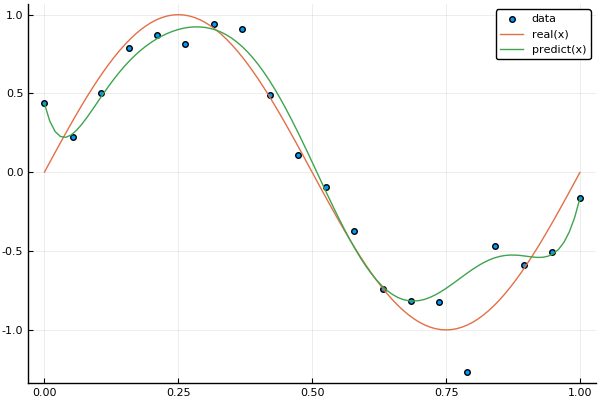
\includegraphics[width=0.9\linewidth]{media/20/ResolveNoLambda}
		\caption{解析法无正则项:误差0.103} %0.10339014377910527
		\label{fig:resolvenolambda20}
	\end{minipage}
	\begin{minipage}[c]{0.5\linewidth}
		\centering
		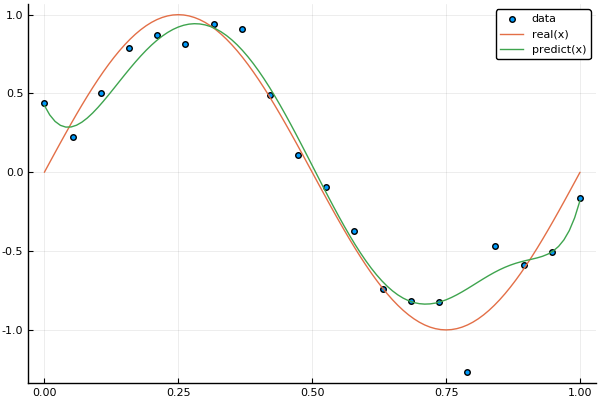
\includegraphics[width=0.9\linewidth]{media/20/ResolveWithLambda}
		\caption{解析法有正则项:误差0.0759} %0.07592688087874981
		\label{fig:resolvewithlambda20}
	\end{minipage}
\end{figure}

\begin{figure}[H]
	\begin{minipage}[c]{0.5\linewidth}
		\centering
		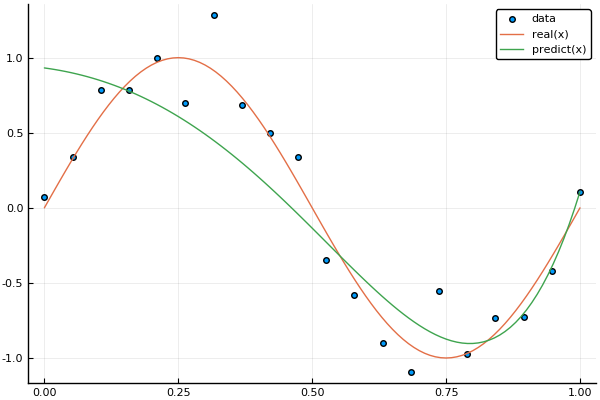
\includegraphics[width=0.9\linewidth]{media/20/SGDNoLambda}
		\caption{梯度下降无正则项:误差0.3023} %0.30229266380909836
		\label{fig:sgdnolambda20}
	\end{minipage}
	\begin{minipage}[c]{0.5\linewidth}
		\centering
		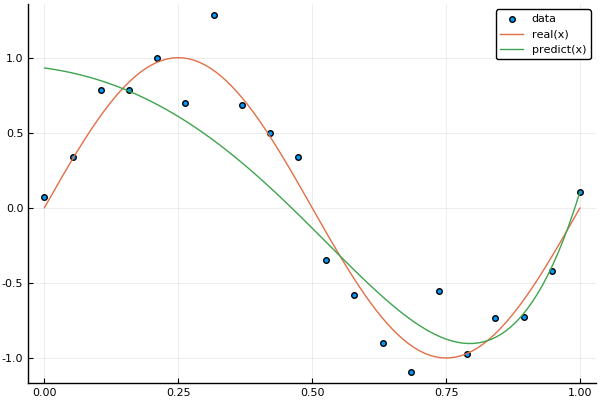
\includegraphics[width=0.9\linewidth]{media/20/SGDWithLambda}
		\caption{梯度下降有正则项:误差0.3021} %0.30212779749293056
		\label{fig:sgdwithlambda20}
	\end{minipage}
\end{figure}

\begin{figure}[H]
	\begin{minipage}[c]{0.5\linewidth}
		\centering
		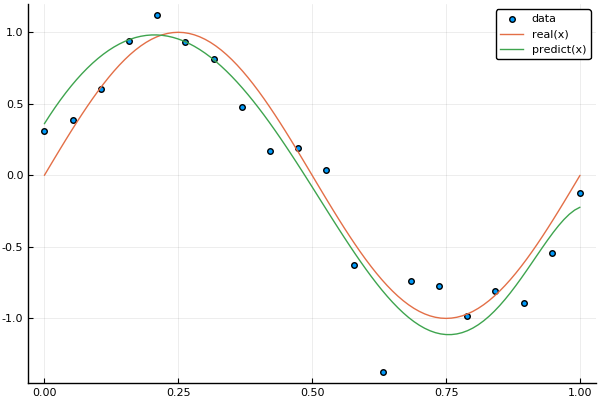
\includegraphics[width=0.9\linewidth]{media/20/ConjugationNoLambda}
		\caption{共轭梯度下降无正则项:误差0.0298} %0.029843459768788647
		\label{fig:connolambda20}
	\end{minipage}
	\begin{minipage}[c]{0.5\linewidth}
		\centering
		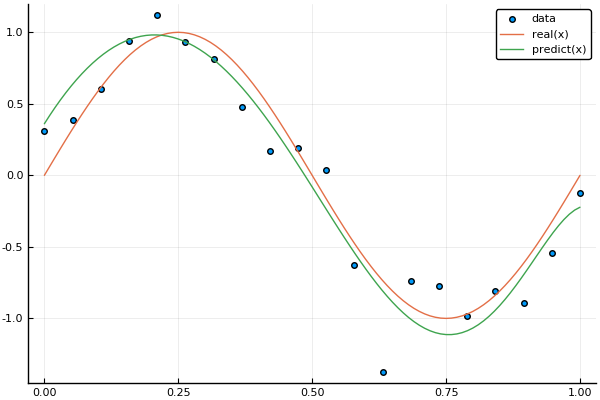
\includegraphics[width=0.9\linewidth]{media/20/ConjugationWithLambda}
		\caption{共轭下降有正则项:误差0.0298} %0.02984362509778699
		\label{fig:conwithlambda20}
	\end{minipage}
\end{figure}

加入正则项带来的效果还是非常明显的。

% -----------------------------------------------------

\begin{figure}[H]
	\begin{minipage}[c]{0.5\linewidth}
		\centering
		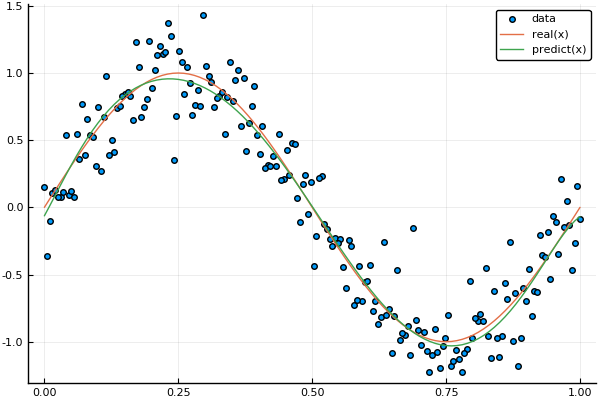
\includegraphics[width=0.9\linewidth]{media/200/ResolveNoLambda}
		\caption{解析法无正则项:误差0.0479} %0.04793831346328907
		\label{fig:resolvenolambda200}
	\end{minipage}
	\begin{minipage}[c]{0.5\linewidth}
		\centering
		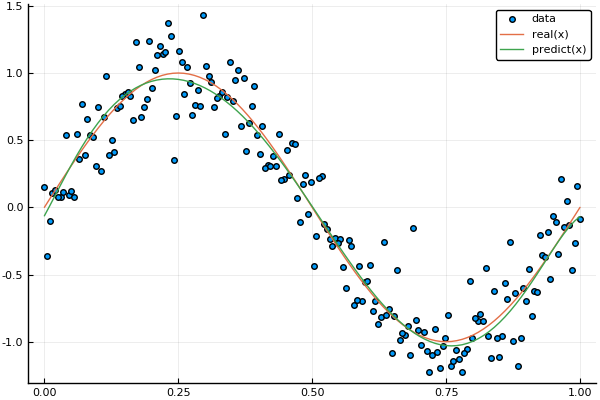
\includegraphics[width=0.9\linewidth]{media/200/ResolveWithLambda}
		\caption{解析法有正则项:误差0.0479} %0.04793355476026563
		\label{fig:resolvenolambda200}
	\end{minipage}
\end{figure}

\begin{figure}[H]
	\begin{minipage}[c]{0.5\linewidth}
		\centering
		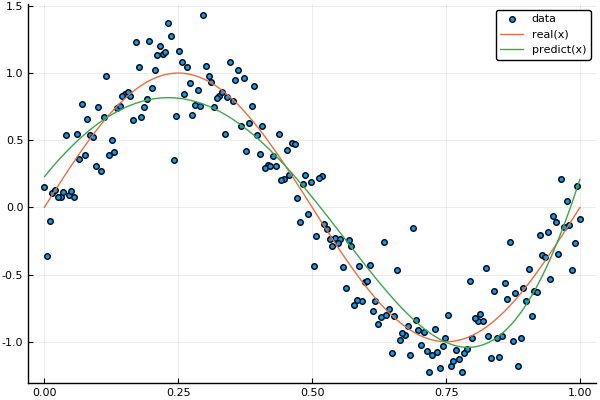
\includegraphics[width=0.9\linewidth]{media/200/SGDNoLambda}
		\caption{梯度下降无正则项:误差0.0668} %0.06679366620364305
		\label{fig:sgdnolambda200}
	\end{minipage}
	\begin{minipage}[c]{0.5\linewidth}
		\centering
		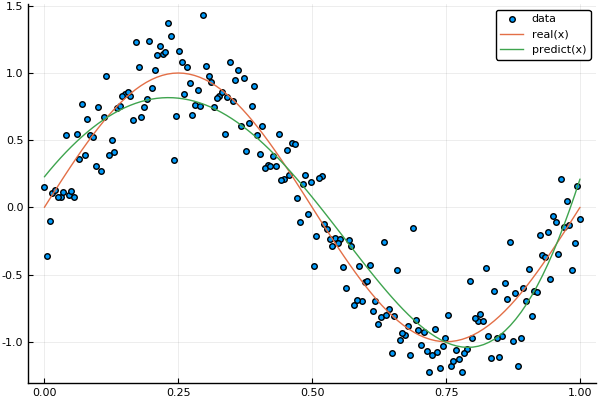
\includegraphics[width=0.9\linewidth]{media/200/SGDWithLambda}
		\caption{梯度下降有正则项:误差0.0667} %0.0667462681749804
		\label{fig:sgdwithlambda200}
	\end{minipage}
\end{figure}

\begin{figure}[H]
	\begin{minipage}[c]{0.5\linewidth}
		\centering
		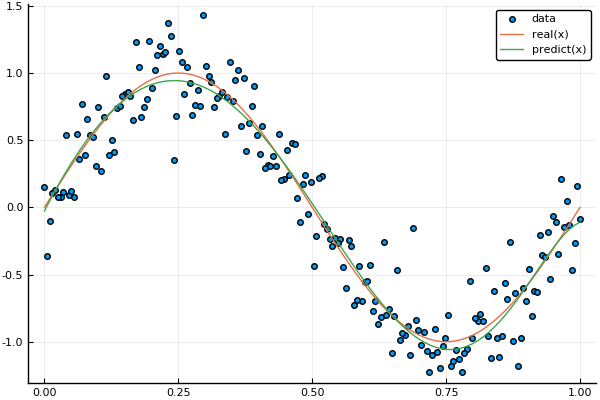
\includegraphics[width=0.9\linewidth]{media/200/ConjugationNoLambda}
		\caption{共轭梯度下降无正则项:误差0.0477} %0.047706040530059425
		\label{fig:connolambda200}
	\end{minipage}
	\begin{minipage}[c]{0.5\linewidth}
		\centering
		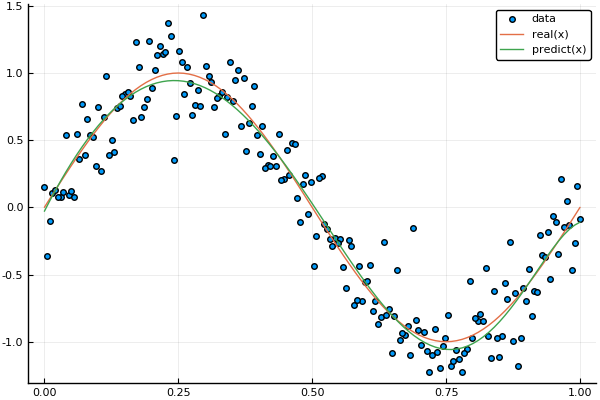
\includegraphics[width=0.9\linewidth]{media/200/ConjugationWithLambda}
		\caption{共轭下降有正则项:误差0.0477} %0.04770591855243747
		\label{fig:conwithlambda200}
	\end{minipage}
\end{figure}

此时误差非常小了,正则项的影响不大了。

% ------------------------------------------------------------------------

\begin{figure}[H]
	\begin{minipage}[c]{0.5\linewidth}
		\centering
		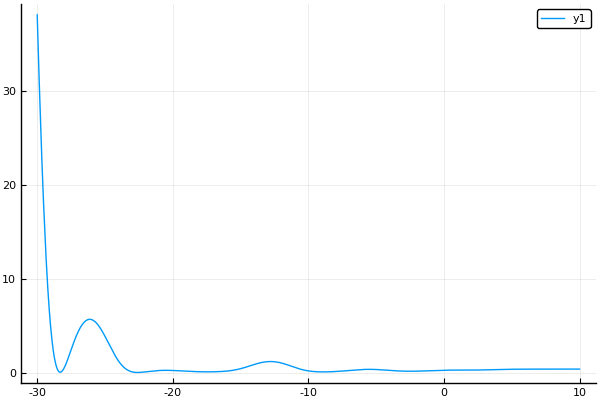
\includegraphics[width=0.9\linewidth]{media/20/ResolveWithLambda-lambda-err}
		\caption{20数据点$\lambda$取值影响}
		\label{fig:resolvelambdaerr20}
	\end{minipage}
	\begin{minipage}[c]{0.5\linewidth}
		\centering
		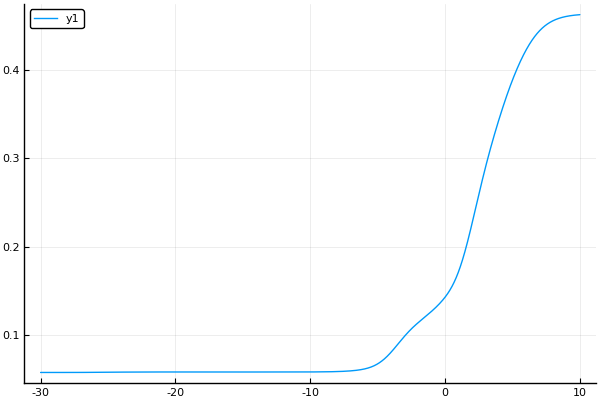
\includegraphics[width=0.9\linewidth]{media/200/ResolveWithLambda-lambda-err}
		\caption{200数据点$\lambda$取值影响}
		\label{fig:resolvelambdaerr200}
	\end{minipage}
\end{figure}

\begin{figure}[H]
	\begin{minipage}[c]{0.5\linewidth}
		\centering
		\includegraphics[width=0.9\linewidth]{media/20/SGDWithLambda-Lambda-err}
		\caption{20数据点$\lambda$取值影响}
		\label{fig:sgdlambdaerr20}
	\end{minipage}
	\begin{minipage}[c]{0.5\linewidth}
		\centering
		\includegraphics[width=0.9\linewidth]{media/200/SGDWithLambda-Lambda-err}
		\caption{200数据点$\lambda$取值影响}
		\label{fig:sgdlambdaerr200}
	\end{minipage}
\end{figure}

\begin{figure}[H]
	\begin{minipage}[c]{0.5\linewidth}
		\centering
		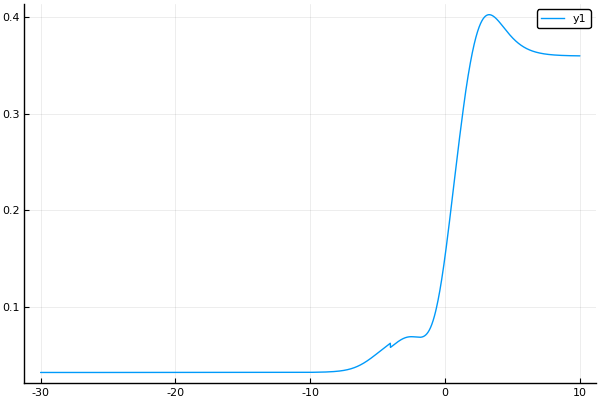
\includegraphics[width=0.9\linewidth]{media/20/ConjugationWithLambda-Lambda-err}
		\caption{20数据点$\lambda$取值影响}
		\label{fig:conlambdaerr20}
	\end{minipage}
	\begin{minipage}[c]{0.5\linewidth}
		\centering
		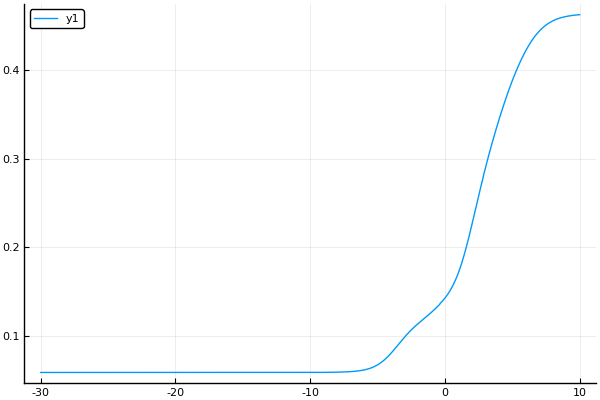
\includegraphics[width=0.9\linewidth]{media/200/ConjugationWithLambda-Lambda-err}
		\caption{200数据点$\lambda$取值影响}
		\label{fig:conlambdaerr200}
	\end{minipage}
\end{figure}

数据量小的时候,正则项的影响相对来说比较明显,这里的数据其实不太好,看起来不太明显,事实上在我之前的多次实验中,有有一些是对比非常明显的。

\section{结论}


数据量越大,我们预测结果的误差就越小,正则项的优化越不明显。

数据量越小越容易出现过拟合,此时加入正则项一定程度上可以解决此问题。

也就是说,在我们训练的时候,如果数据量比较大,正则项是可有可无的,而在数据比较少的时候,限制模型的复杂度就显得非常重要了。同时上面的现象也说明了为什么机器学习是在计算机速度发展到今天的速度以及数据量如此之大的时候发展的如此迅猛。

\begin{thebibliography}{0}
    \addcontentsline{toc}{section}{参考文献}
    \bibitem{共轭梯度法} 维基百科,{\it \href{https://zh.wikipedia.org/wiki/共轭梯度法}{共轭梯度法词条}}
\end{thebibliography}

\appendix

\section{源代码}

\inputminted[breaklines=true,frame=lines,mathescape=true]{julia}{../LinnerModel.jl}

\end{document}
